\documentclass[10pt]{article}

\usepackage{listings}
\usepackage{graphicx}
\usepackage{psfrag}
\usepackage{amssymb}

\usepackage{caption}
\usepackage{subcaption}
\renewcommand\thesubfigure{Fig.\alph{subfigure}}

\usepackage{fullpage}


%opening
\title{CayMos User Manual: \\User Interface, Functionalities and Pseudocode}

\author{Menghan Wang and Meera Sitharam \\ University of Florida}

 
\begin{document}

\maketitle

\texttt{CayMos}~\cite{bib:caymos} is a software system for analyzing the configuration spaces  of a common class of 2D mechanisms called 1-dof tree decomposable linkages with low Cayley complexity~\cite{Sitharam2011a}.
\texttt{CayMos} implements efficient algorithmic solutions for: (a) meaningfully representing and visualizing the connected components of the Euclidean realization space of the linkage; (b) finding a path of continuous motion between two realizations in the same connected component, with or without restricting the realization type (sometimes called orientation type); (c) finding two ``closest'' realizations in different connected components. 


\section{\texttt{CayMos} Functionalities and User Interface}

\texttt{CayMos} accepts user input of a linkage by 
allowing the user to draw the bar and joints of the linkage. 


%ODO REFER TO EXAMPLE SCREENSHOT?


%-----------------------

\subsection{Generating Cayley configuration spaces}\label{subsec:ccs}



The user can generate the Cayley configuration spaces for 1-dof tree-decomposable linkages with low Cayley complexity. 
The following functionalities are provided by \texttt{CayMos}: 

\begin{enumerate}


\item \texttt{CayMos} determines whether the given linkage is 1-dof tree-decomposable. 
For a 1-dof tree-decomposable linkage, 
it determines whether the linkage has low Cayley complexity, implementing the Four-cycle algorithm from \cite{Sitharam2011b}. 

\item For a linkage with low Cayley complexity, \texttt{CayMos} generates both the oriented and non-oriented Cayley configuration space(s), 
implementing the ELR algorithm from \cite{Sitharam2011a}.
See Figure \ref{fig:ccs} and \ref{fig:occs} for the user interface. 

%Here user can choose between non-oriented or oriented mode. 

\item The user can change the length of the chosen base non-edge to see corresponding realizations.
The generated Cayley configuration space is shown as a set of intervals, 
and a dot representing the current Cayley configuration is shown on the axis, 
as shown in Figure \ref{fig:ccs} (C).
The user can use a spinner to change the Cayley configuration and show 
 a corresponding realization, 
 as shown in Figure \ref{fig:ccs} (B). % corresponding to current Cayley configuration will be shown. 

\item The user can specify the realization type by changing the local orientations at specified construction steps.
The realizations shown, as well as the intervals of the oriented Cayley configuration spaces, are color-coded corresponding to different realization types.
See Figure \ref{fig:occs}. 

\end{enumerate}

\begin{figure*}[hbtp]
\begin{center}
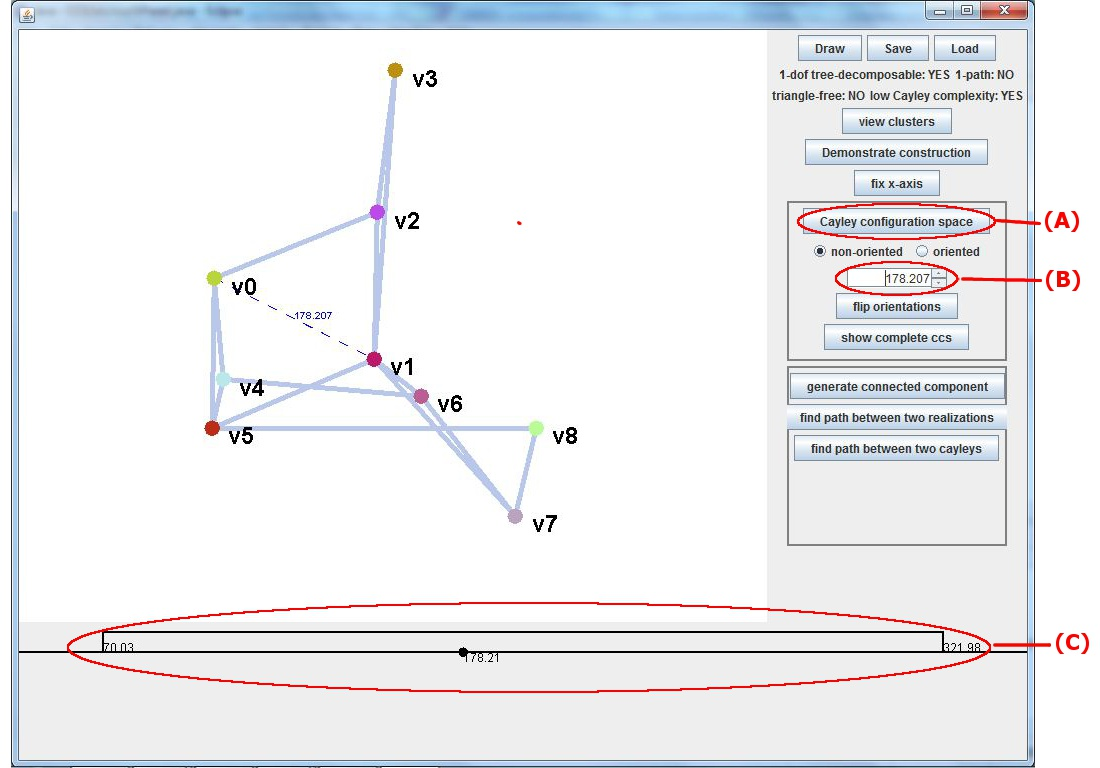
\includegraphics[width=0.65\linewidth]{img/ccs}
\end{center}
\caption{Generating the non-oriented Cayley configuration space of the Limacon linkage using \texttt{CayMos}. 
(A) Button for generating the Cayley configuration space. 
(B) Spinner for specifying the length of the base non-edge and navigating the Cayley configuration space. 
(C) Intervals of the Cayley configuration space. The black dot denotes the Cayley configuration for the current realization. }
\label{fig:ccs}
\end{figure*}

\begin{figure*}[hbtp] 
\centering
\begin{subfigure}[b]{0.65\linewidth}
\centering
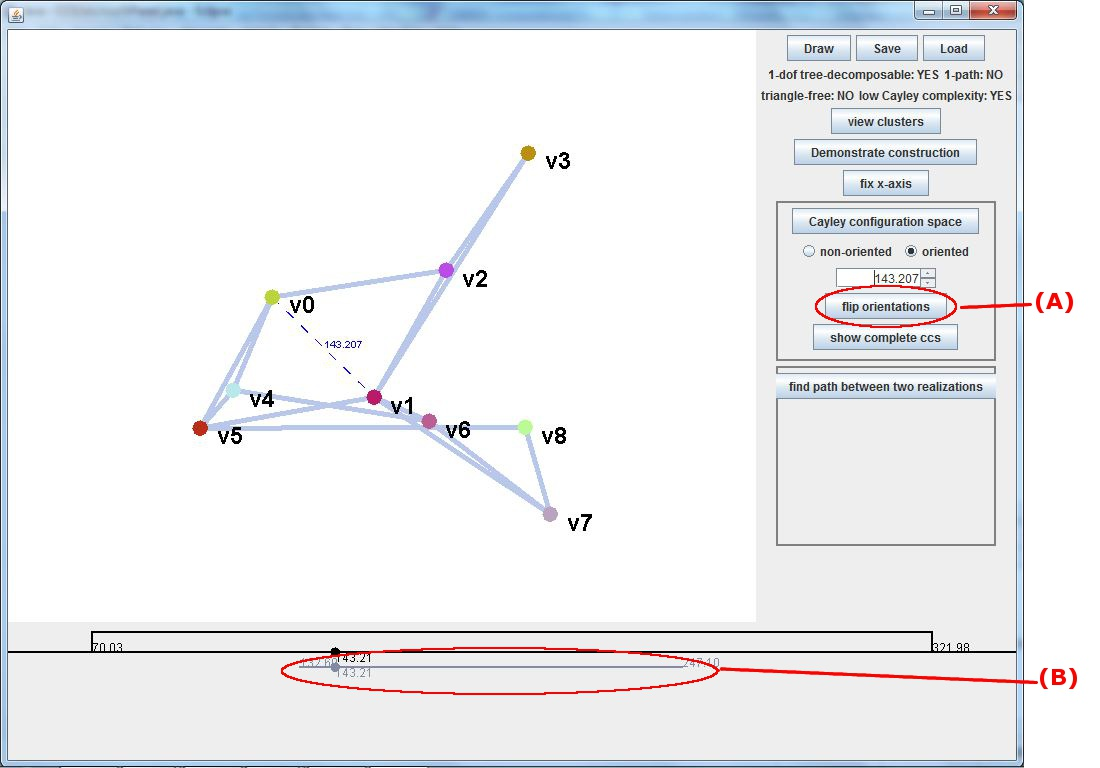
\includegraphics[width=1.1\textwidth]{img/occs1}
\caption{}
%\label{fig:cardioid}
\end{subfigure}
%
\begin{subfigure}[b]{0.65\linewidth}
\centering
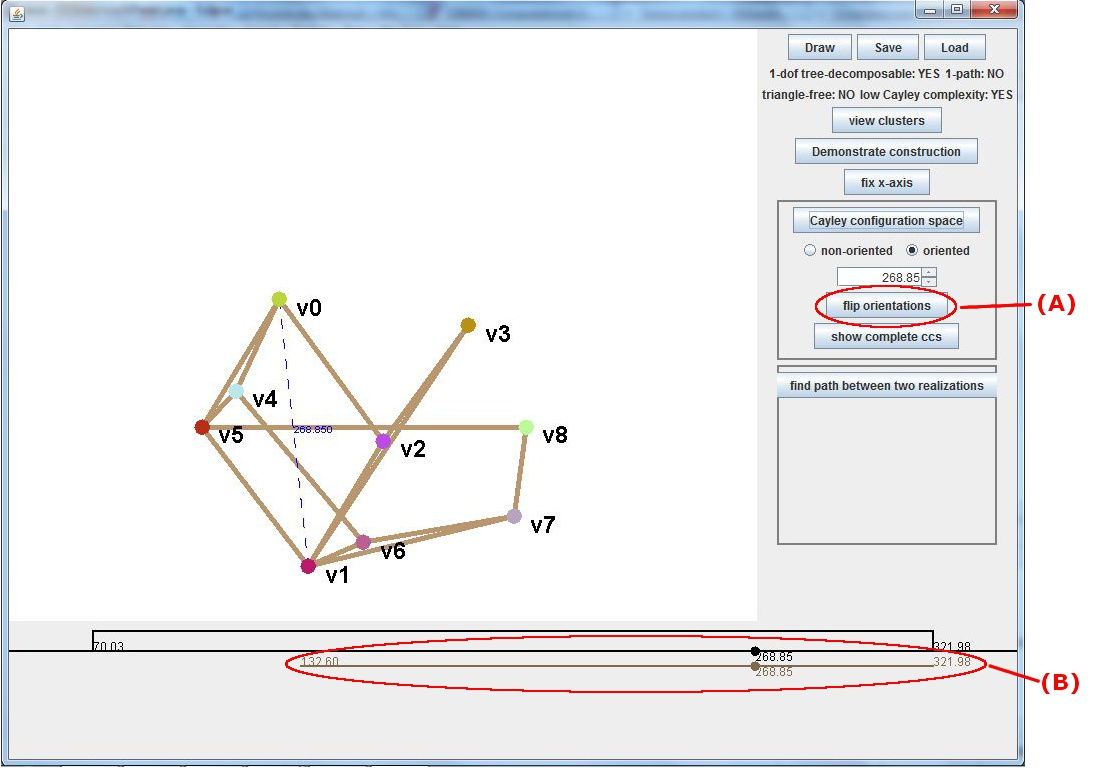
\includegraphics[width=1.1\textwidth]{img/occs2}
\caption{}
%\label{fig:limacon}
\end{subfigure}
\caption{Two different oriented Cayley configuration spaces of the Limacon linkage. 
(A) Button for changing the realization type. 
(B) Intervals of the corresponding oriented Cayley configuration space.  }
\label{fig:occs}
\end{figure*}



%--------------------------


\subsection{Visualizing a connected component of the realization space}\label{subsec:connected_component}


After generating the Cayley configuration space, 
the user can generate and visualize the connected component of the realization space containing a given realization. 
The following functionalities are provided by \texttt{CayMos}:  

\begin{enumerate}

\item Showing the non-edges in the complete Cayley vector of the linkage, 
as well as displaying the complete Cayley distance vector for the current realization. 
See Figure \ref{fig:components} (B) and (C). 

\noindent\textbf{Note:} The current version of the software implements the complete Cayley vector defined in \cite{sitharam2014beast}, which has higher dimension than the \emph{minimal complete Cayley vector} defined in \cite{Sitharam2011a}.

\item Generating the connected component containing the current realization, 
%as well as all connected components of the realization space,
implementing the Continuous motion path algorithm from \cite{Sitharam2011a}.
See Figure \ref{fig:components} (A). 
%Allow user to navigate each component. 


\item Visualizing the connected component: 
the user can pick three non-edges from the complete Cayley vector, 
and \texttt{CayMos} shows the 3D projection of the canonical Cayley curve of the current connected component on those three non-edges. 
\texttt{CayMos} permits the user to use a spinner to trace the connected component, 
and a moving dot is shown on the curve to denote the current realization.
The canonical Cayley curve is color-coded corresponding to realization types encountered in the connected component. 
See Figure \ref{fig:components} (E), (G) and (D). 
%Visualizes the connected component by  showing the projection of the

\item Showing the intervals of oriented Cayley configuration spaces contained in the current connected component. 
The intervals are color-coded corresponding to realization types. 
See Figure \ref{fig:components} (H). 

\item Showing the curves traced out by vertices of the linkage in the current connected component. 
See Figure~\ref{fig:tracing}.

\end{enumerate}

\begin{figure*}[hbtp] 

\centering
\begin{subfigure}[b]{\linewidth}
\begin{center}
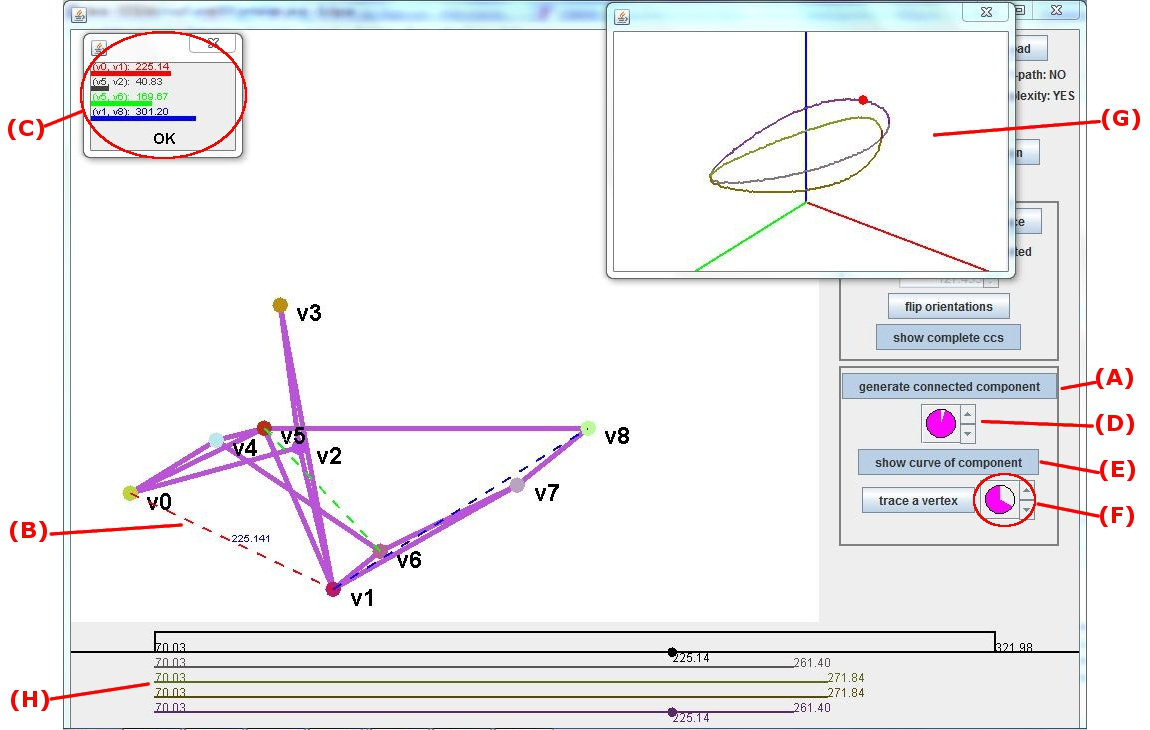
\includegraphics[width=.65\textwidth]{img/component1}
\end{center}
\caption{}
%\label{fig:cardioid}
\end{subfigure}
%
%\begin{subfigure}[b]{0.49\linewidth}
%\centering
%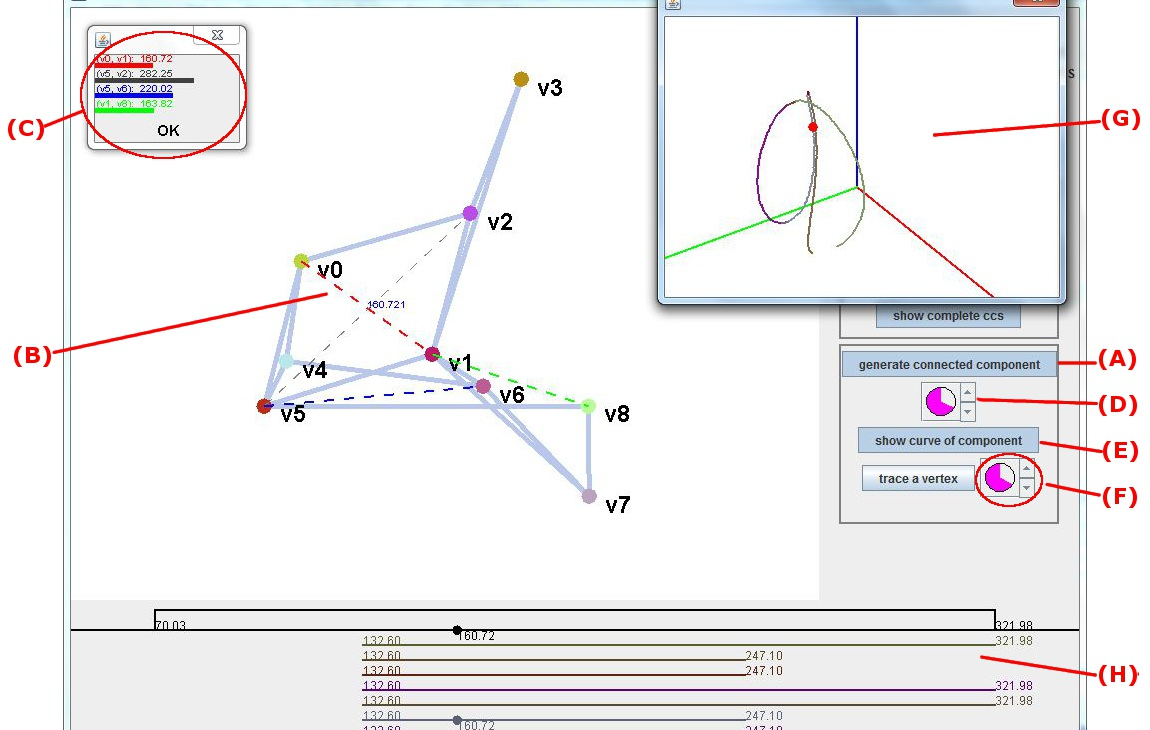
\includegraphics[width=0.9\textwidth]{img/component2}
%\caption{}
%%\label{fig:limacon}
%\end{subfigure}
\begin{subfigure}[b]{\linewidth}
\begin{center}
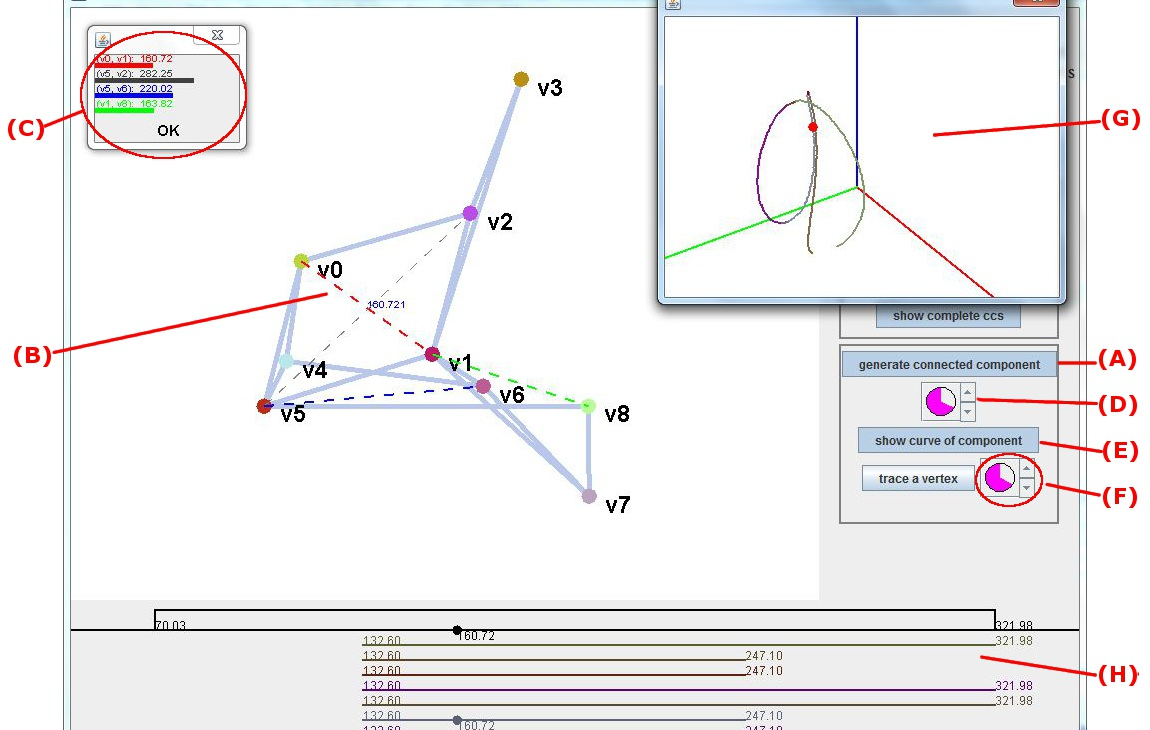
\includegraphics[width=.65\textwidth]{img/component2}
\end{center}
\caption{}
%\label{fig:limacon}
\end{subfigure}
\caption{Finding the connected components and showing corresponding canonical Cayley curves of 
the Limacon linkage using \texttt{CayMos}, where (Fig.a) and (Fig.b) show two different connected components. 
(A) Button for generating the connected components. 
(B) The current realization, moving as the user traces the connected component. Dashed non-edges: non-edges in the complete Cayley vector. 
(C) Panel showing the complete Cayley distance vector for current realization. 
\texttt{CayMos} allows the user to pick three non-edges for 3D projection of the canonical Cayley curve,  
where the picked non-edges are shown in red, green and blue in (B) and (C). 
(D) Spinner for tracing the current connected component. 
(E) Button for showing the 3D projection of the corresponding canonical Cayley curve. 
(F) Spinner for navigating all connected components in the realization space. 
(G) The 3D projection of the canonical Cayley curve of the current component. 
The dot denotes the current realization and moves as the user traces the connected component. 
The curve is color-coded according to realization types. 
(H) The intervals of the oriented Cayley configuration spaces contained in the current connected component. }
\label{fig:components}
\end{figure*}

\begin{figure*}[hbtp]
\begin{center}
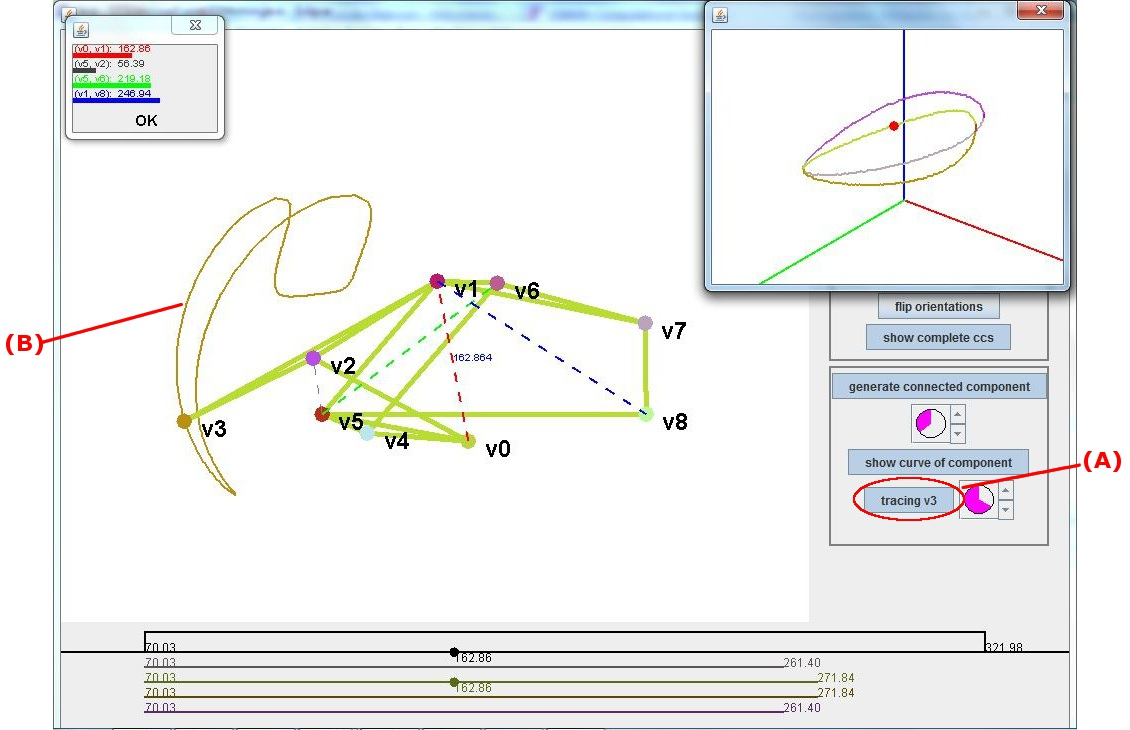
\includegraphics[width=.65\linewidth]{img/tracing}
\end{center}
\caption{
Showing the curve traced out by a vertex in a non-standard component of the Limacon linkage.   
(A) Button for tracing a vertex. 
(B) The curve traced by the selected vertex.}
\label{fig:tracing}
\end{figure*}



\subsection{All connected components and continuous paths in the realization space}\label{subsec:path}

The user can generate all connected components of the realization space, and find a continuous motion path between two realizations. 
%and find the Cayley distance between two realizations in different connected components. 
The following functionalities are provided by \texttt{CayMos}: 

\begin{enumerate}

\item Generating all connected components of the realization space,
implementing the adapted Continuous motion path algorithm from \cite{sitharam2014beast}.
See Figure \ref{fig:components}  (F). 
%Allow user to navigate each component. 

\item Finding a continuous path between two realizations specified by the user (if one exists),
implementing the Continuous motion path algorithm from \cite{Sitharam2011a}.
See Figure \ref{fig:paths} (Fig.a). 

%The connected component containing the path is shown as a projected 3D curve,  
%and the path is marked on the curve. 
%\item Continuous Path between Cayley configurations: \\
%Finds a continuous path between  two given Cayley configurations (if one exists),
%implementing algorithm from \cite{Sitharam2011a}.

\item Finding a continuous path between two given realizations,
maintaining the same realization type.
Note that such a path exists if and only if those two realizations lie in the same interval in the oriented Cayley configuration space \cite{Sitharam2011a}. 
See Figure \ref{fig:paths} (Fig.b). 


\end{enumerate}


\begin{figure*}[hbtp] 
\centering
\begin{subfigure}[b]{\linewidth}
\centering
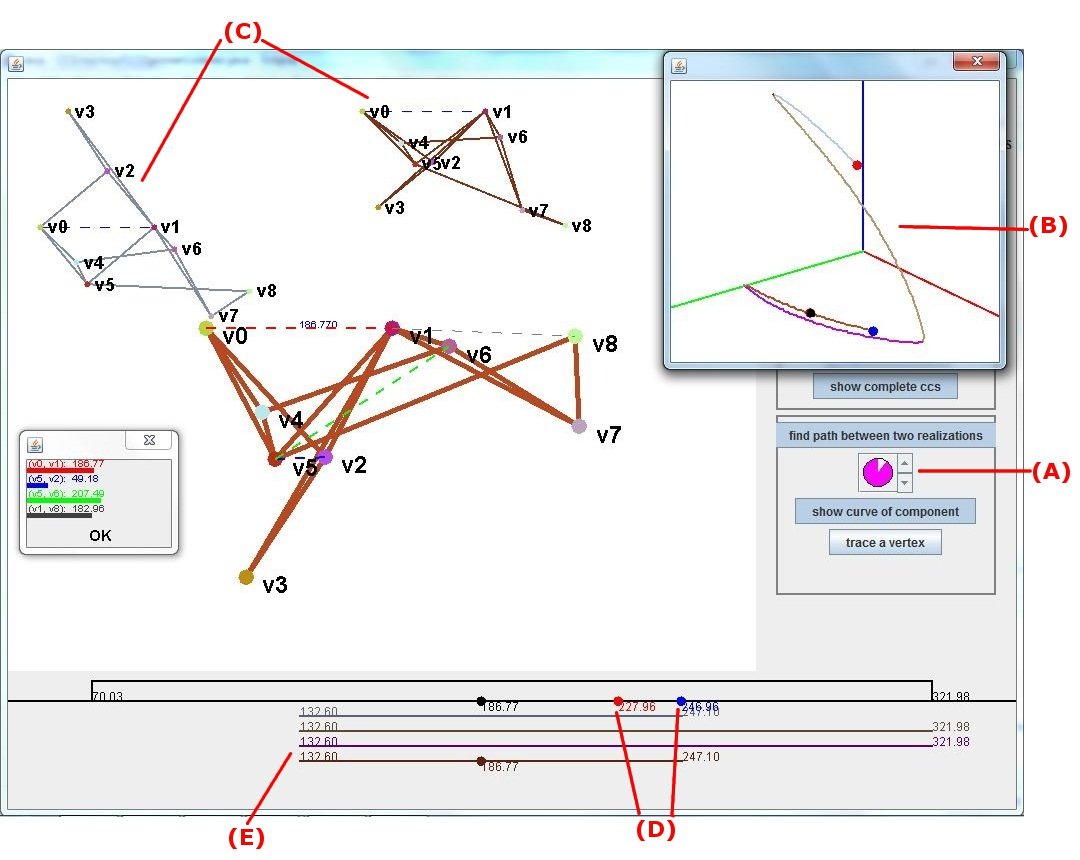
\includegraphics[width=.65\textwidth]{img/path}
\caption{}
%\label{fig:cardioid}
\end{subfigure}
%
\begin{subfigure}[b]{\linewidth}
\centering
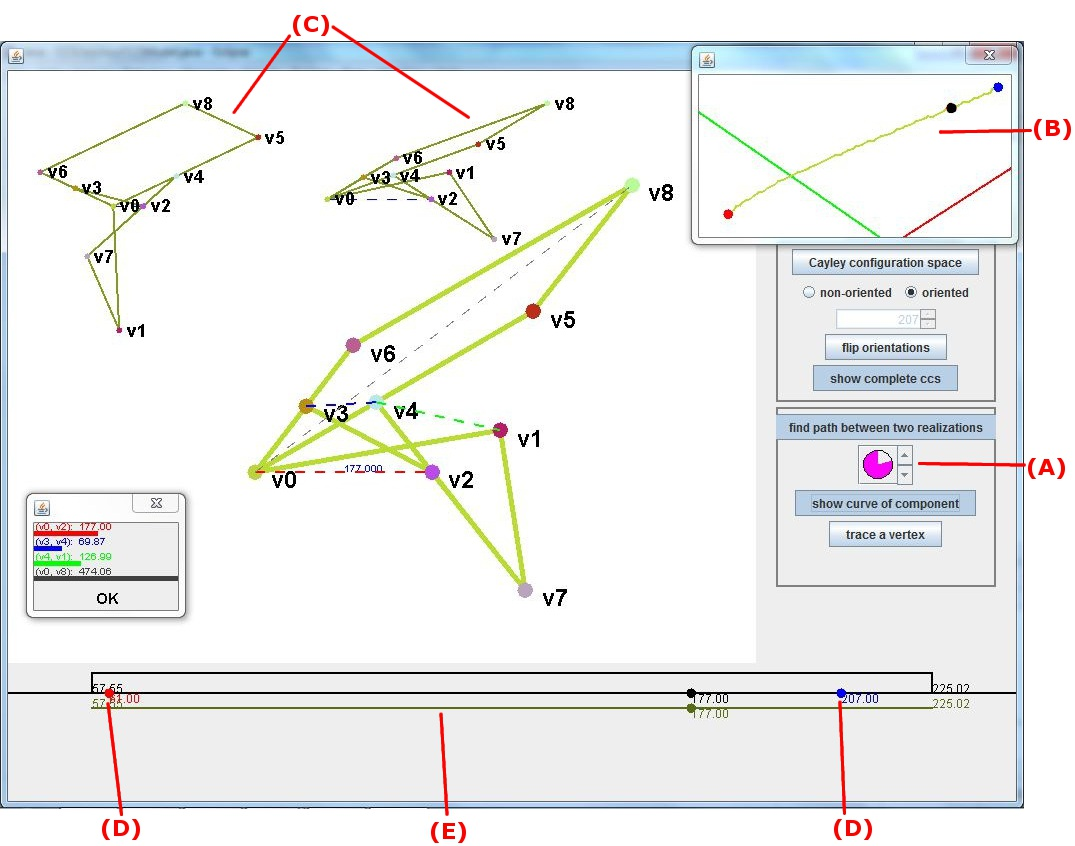
\includegraphics[width=.65\textwidth]{img/opath}
\caption{}
%\label{fig:limacon}
\end{subfigure}

\caption{(Fig.a) Finding a continuous motion path between two realizations of the Limacon linkage. 
(Fig.b) Finding a continuous motion path maintaining the same realization type between two realizations of the Cadioid linkage. 
(A) Spinner for tracing the generated continuous motion path. 
(B) The 3D projection of the segment of the canonical Cayley curve corresponding to the continuous motion path. 
The red and blue dots denote the start and end realizations. 
The black dot denotes the current realization and moves as the user traces the path. 
(C) The start and end realizations.
(D) The Cayley configuration for the start and end realizations.
(E) The intervals of the oriented Cayley configuration spaces encountered along the path. }
\label{fig:paths}
\end{figure*}



\subsection{Cayley distance between connected components}\label{subsec:distance}


When the user specifies two realizations in different connected components and
tries to find a continuous motion path between them, 
\texttt{CayMos} will
%generate the connected components for both realizations and 
find the two nearest realizations of these two components using the Closest pair algorithm from \cite{sitharam2014beast}. 
Both connected components are shown as projected curves, 
and the two nearest realizations are marked on the two curves. 
See Figure \ref{fig:nopath}. 


\begin{figure*}[hbtp]
\begin{center}
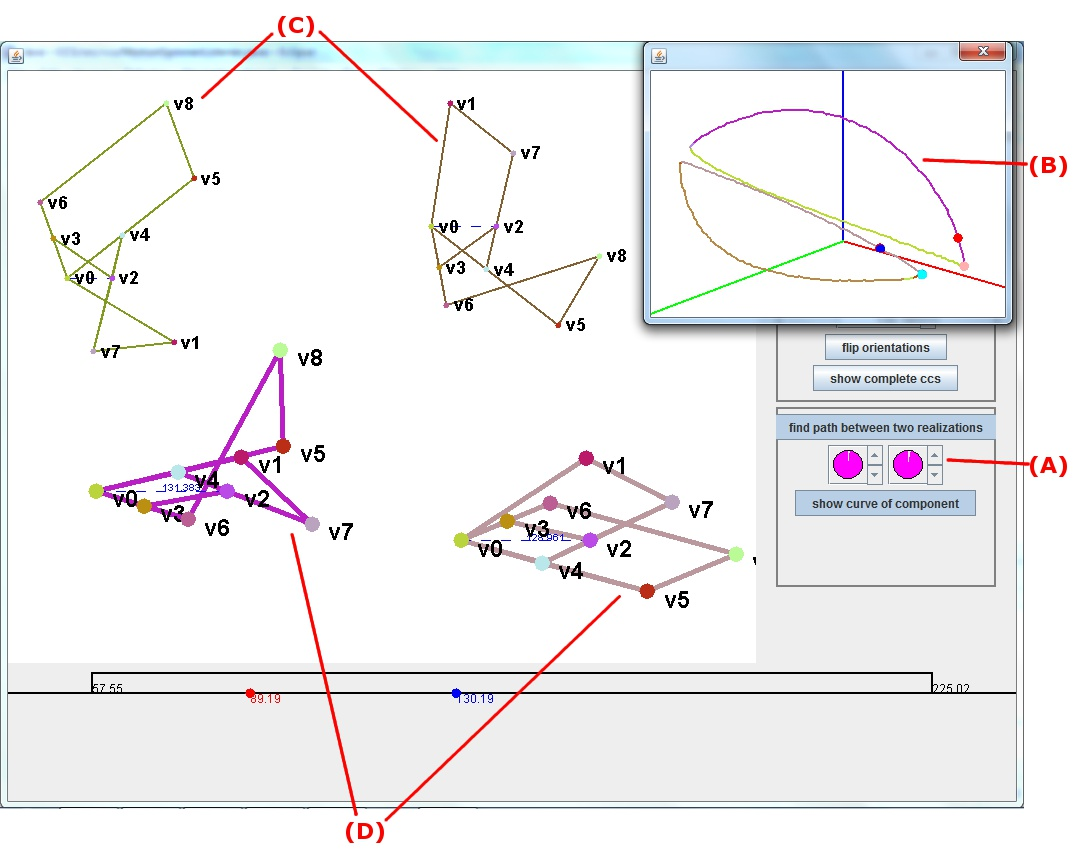
\includegraphics[width=.65\linewidth]{img/nopath}
\end{center}
\caption{Finding two nearest realizations between two connected components using \texttt{CayMos}.  
%1. Button for finding the continuous motion path between two realizations, 
(A) Spinners for tracing the two connected components containing the two given realizations. 
(B) The 3D projection of the corresponding Cayley curves of both connected components. 
The pink and cyan dots denote the two nearest realizations between the two components. 
The red and blue dots denote the current realizations and moves when tracing two components. 
(C) The start and end realizations. 
(D) The current realizations represented and traced by moving dots on the two components. % for tracing the two components.
 }
\label{fig:nopath}
\end{figure*}




\section{\texttt{CayMos} software architecture and pseudocode}




\subsection{Major classes and architecture of \texttt{CayMos}}
\label{sec:classes}



Overall the backend of \texttt{CayMos} consists of two parts, with the following major classes. 
%The backend of the system can be divided into two parts: 


\subsubsection{1-dof tree-decomposable linkages and Cayley configuration spaces}


\begin{enumerate}


\item The \textsf{TDLinkage} class: represents a 1-dof tree-decomposable linkage. 
%Determines whether a linkage has low Cayley complexity, and generates the Cayley configuration space.



 Major Attributes:

\noindent --  \textsf{graph}: the underlying graph of the linkage. 

\noindent --  \textsf{barLengths}: the length of the bars of the linkage. 

\noindent --  \textsf{baseNonedge}: current base non-edge of the linkage.

\noindent --  \textsf{completeCayleyVector}: the complete Cayley vector for the current base non-edge.

\noindent --  \textsf{cayleyConfigurationSpace}: the Cayley configuration space on the current base non-edge. 

\smallskip
\noindent Major Methods:

\noindent-- \textsf{isLow()}: elaborated in Section \ref{sec:islow}.

\noindent-- \textsf{getCayleyConfigurationSpace()}: elaborated in Section \ref{sec:getcayleyconfigurationspace}.


\item The \textsf{Realization} class: represents a realization of a \textsf{TDLinkage} instance.

\noindent Major Attributes:

\noindent --  \textsf{tdLinkage}:
the corresponding 1-dof tree-decomposable linkage of the realization. 

\noindent --  \textsf{points}:
the 2D points in the realization for the vertices of the linkage. 

\smallskip

\noindent Major Methods:

\noindent --  \textsf{length(e:Edge)}: 
Returns the length of \textsf{e} in the realization, where \textsf{e} can be an edge or a non-edge.

\noindent --  \textsf{getCompleteCayleyDistanceVector}(): 
Returns the complete Cayley distance vector of the realization.
Calls \textsf{length()} for each non-edge in the \textsf{completeCayleyVector} field of \textsf{tdLinkage}, with time complexity $O(|V|)$.

\noindent --  \textsf{cayleyDistance(that:Realization)}: 
Returns the Cayley distance \cite[Section 3.2]{sitharam2014beast} between this realization and \textsf{that} with time complexity $O(|V|)$.



\item The \textsf{CayleyConfigurationSpace} and \textsf{OrientedCayleyConfigurationSpace} classes: represent the Cayley configuration space of a \textsf{TDLinkage} instance. Each \textsf{CayleyConfigurationSpace} contains multiple \textsf{OrientedCayleyConfigurationSpace} instances. 

\item The \textsf{OrientedInterval} class: represents an interval in an oriented Cayley configuration space. 

\noindent Major Attributes:

\noindent -- \textsf{upper} and \textsf{lower}:
the upper and lower endpoints of the interval.

\noindent --  \textsf{realizationType}:
the realization type of the \textsf{OrientedCayleyConfigurationSpace} containing the interval.

\noindent --  \textsf{nextIntervalUpper} and \textsf{nextIntervalLower}:
the two \textsf{OrientedInterval} instances sharing a common endpoint with this interval. 
They are immediately reachable from this interval in a continuous motion.


\end{enumerate}



%\item CayleyConfigurationSpace: the Cayley configuration space of a TDLinkage instance on a base non-edge. 
\subsubsection{Continuous motion generation and representation}

\begin{enumerate}


\item The \textsf{ContinuousMotion} class: represents a continuous motion path between two \textsf{Realization} instances, or a connected component of a \textsf{TDLinkage} instance. 


\noindent  Major Attributes:

\noindent -- \textsf{tdLinkage}: 
the corresponding 1-dof tree-decomposable linkage of the continuous motion. 

\noindent --  \textsf{orientedIntervals}: 
the list of \textsf{OrientedInterval} instances encountered along the continuous motion.

\smallskip

\noindent Major methods:

\noindent -- \textsf{findComponent()}, \textsf{findPath()} and \textsf{findAllComponents()}: elaborated in Section~\ref{sec:findpath}.

\noindent -- \textsf{findNearestRealizations()}: elaborated in Section~\ref{sec:findnearest}.


\noindent -- \textsf{getRealizations()}: 
Returns a list of realization samples along the continuous motion by sampling the \textsf{orientedIntervals} field. 
Uses a sampler object so that different ways of sampling can be chosen at runtime. 

\noindent --  \textsf{get3DCurve(f1,f2,f3)}: 
Returns a \textsf{Curve3D} instance representing the 3D projection of the continuous motion's corresponding Cayley curve
on \textsf{f1}, \textsf{f2} and \textsf{f3}, three non-edges from the complete Cayley vector of tdLinkage. 
The time complexity is linear in the size of the list returned by \textsf{getRealizations()}.


\item The \textsf{Curve3D} class: supports visualization of a  \textsf{ContinuousMotion} instance as a Cayley curve projected in 3D.

\end{enumerate}

\begin{figure*}[tp]
\begin{center}
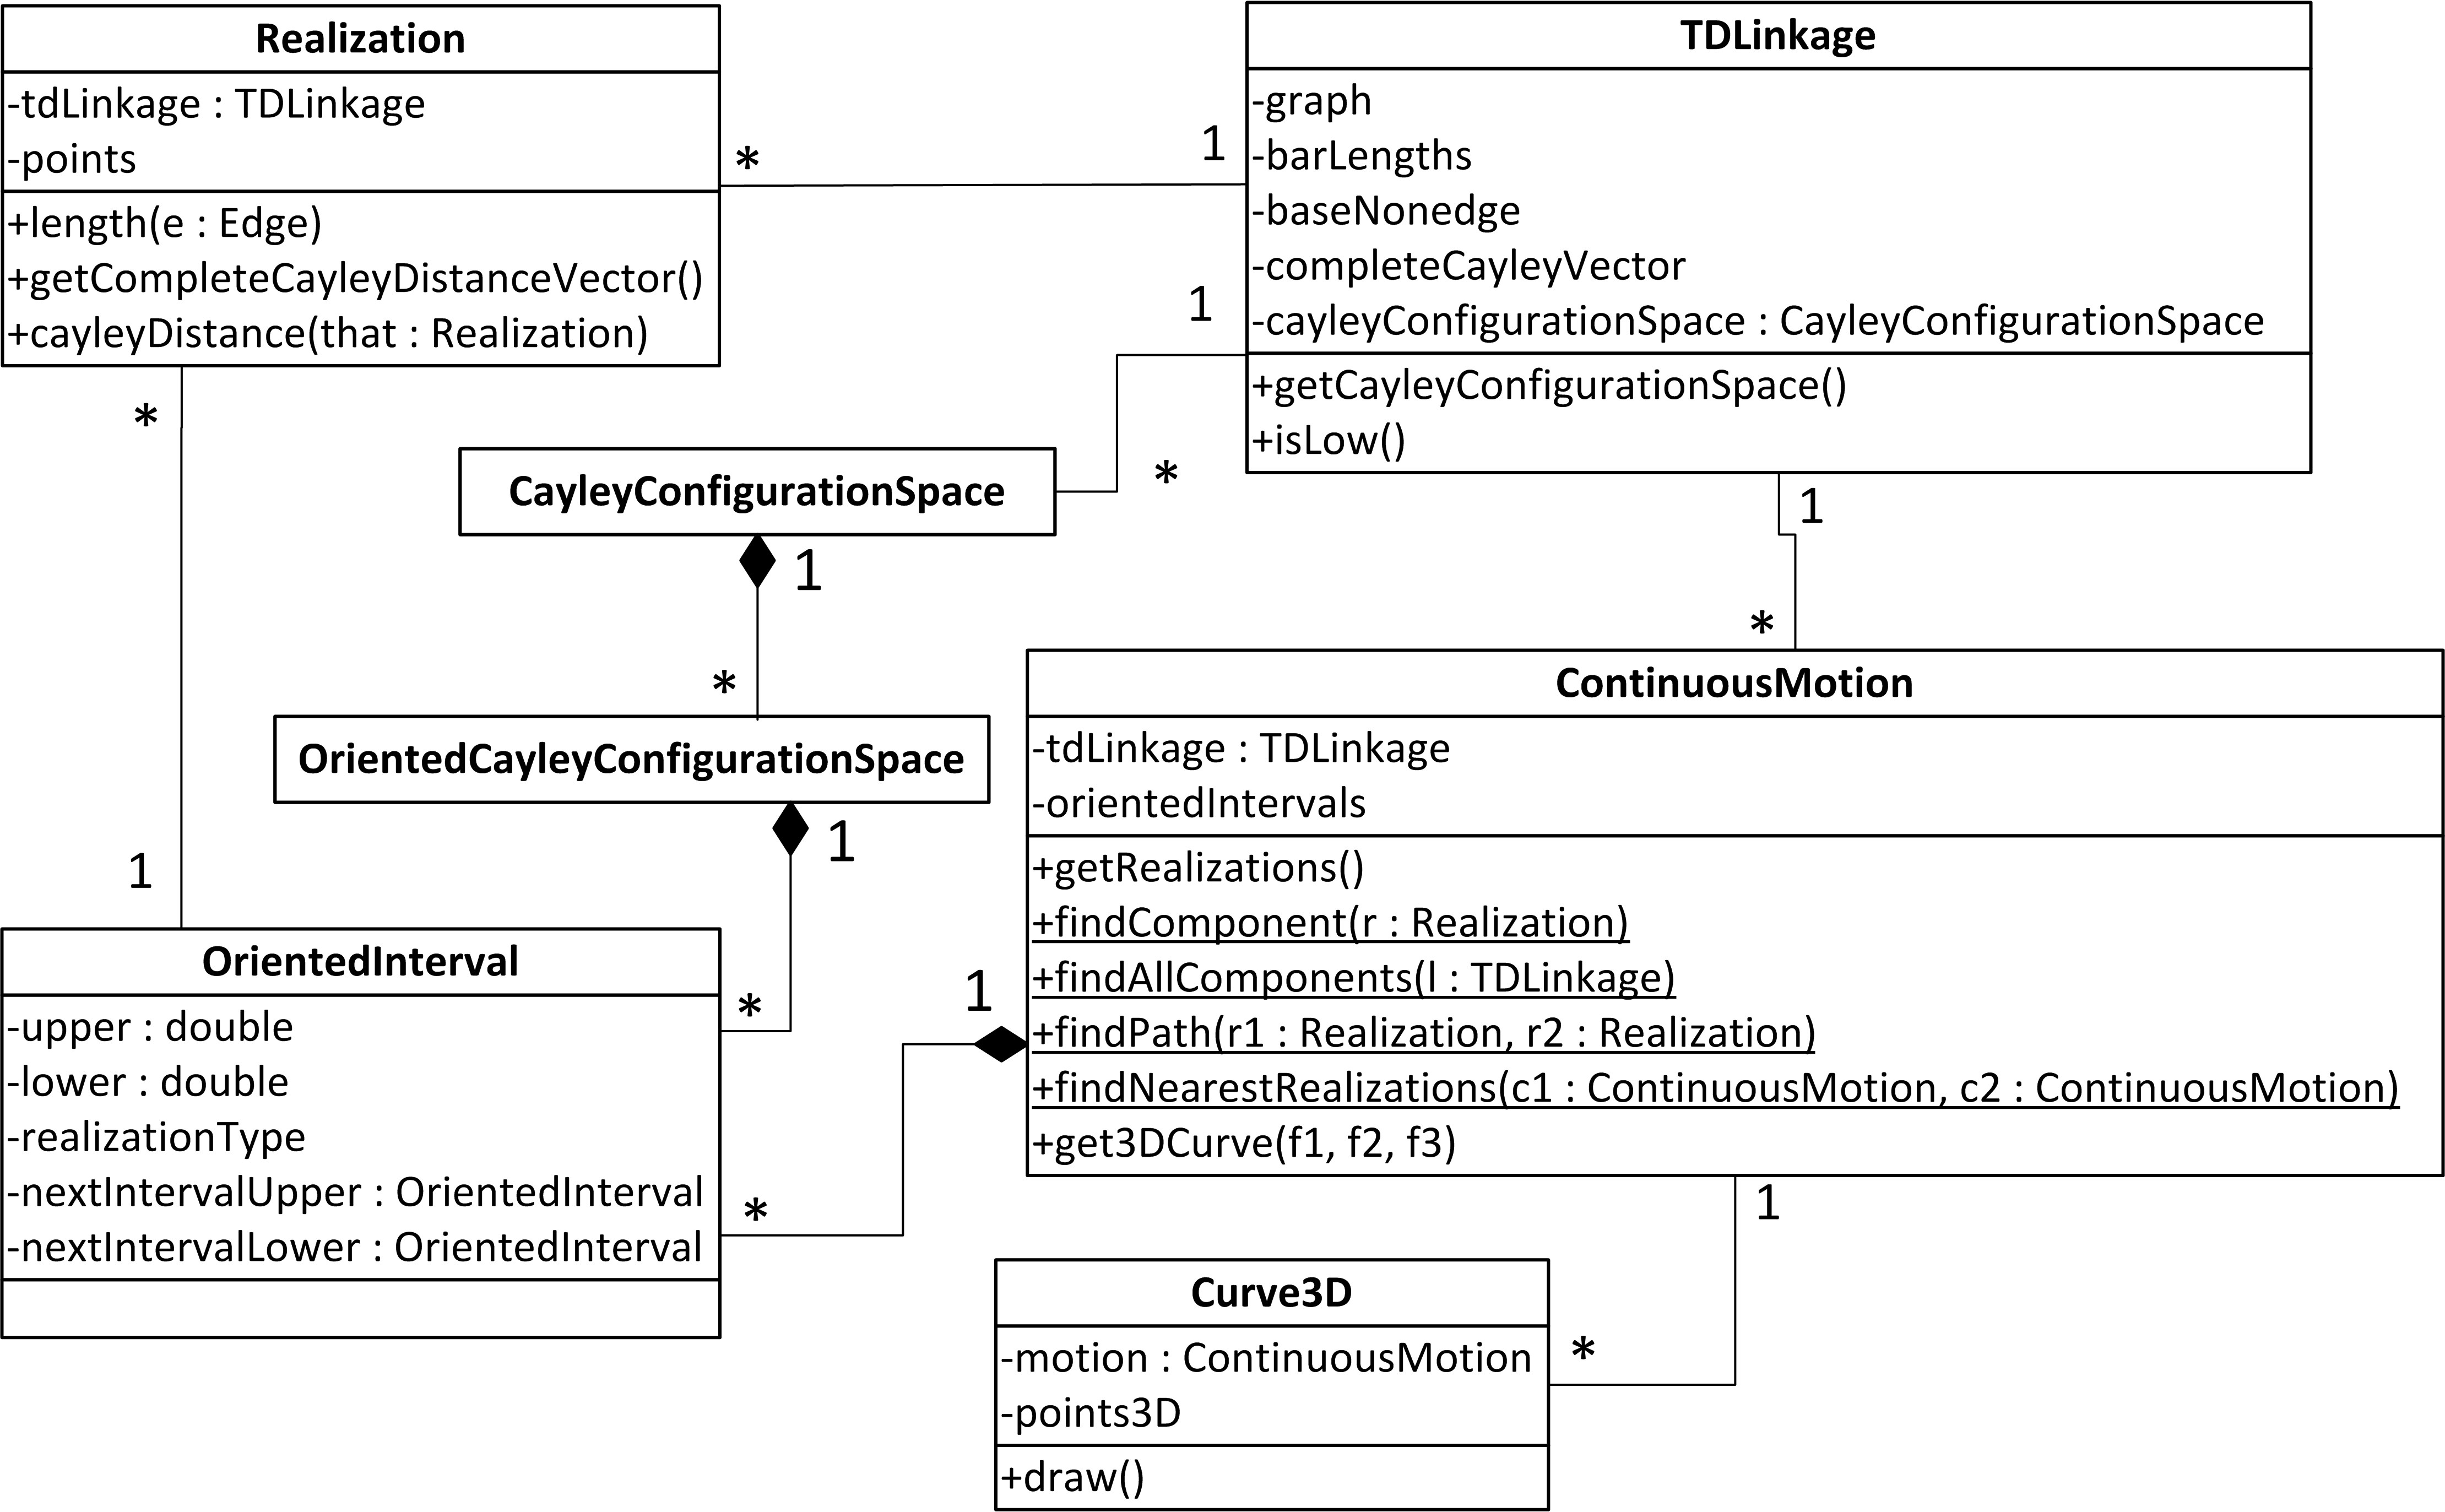
\includegraphics[width=0.8\linewidth]{img/uml}
\end{center}
\caption{UML diagram for major classes. }
\label{fig:uml}
\end{figure*}

Figure \ref{fig:uml} shows the relationships between the above classes. 








%-------------------------------------------------------------------


\subsection{Major methods}
\label{sec:pseudocode}

\subsubsection{ Method \textsf{isLow()}} %implements the Four-cycle algorithm \cite{Sitharam2011b} sketched in Section \ref{sec:algorithms}
\label{sec:islow}

%Returns whether the linkage \textsf{this} has low Cayley complexity. 
%Initializes the \textsf{completeCayleyVector} field, % for linkages with low Cayley complexity,
%which stores the complete Cayley vector for the current base non-edge. 

The method implements the Four-cycle algorithm \cite[Theorem 2]{Sitharam2011b} %sketched in Section \ref{sec:algorithms} to determine low Cayley complexity,
returning \textsf{true} if the calling \textsf{TDLinkage} instance has low Cayley complexity, or \textsf{false} otherwise.
It also implements  \cite[Theorem 3]{sitharam2014beast} to find the complete Cayley vector
and store it in  the  \textsf{completeCayleyVector} field. 
Since both algorithms follow the construction of the linkage, we combine the implementation into one method. 
The  time complexity is $O(|V|^2)$. 

\smallskip
\noindent\textbf{Note:} in the current version of the software, the complete Cayley vector is implemented 
as in \cite[Theorem 3]{sitharam2014beast}, which is not minimal. 
The \emph{minimal complete Cayley vector} introduced in \cite[Theorem 4]{Sitharam2011a} will have dimension two for a large number of 1-dof tree-decomposable linkages. 

\smallskip

\lstset{language=Java} 

\lstset{
  language=Java,
  tabsize=2,
  basicstyle=\footnotesize\sffamily,
  %frame=single,
  breaklines=true
}

 Pseudocode for  \textsf{isLow()} :

\begin{lstlisting}[mathescape]
boolean isLow() {
	completeCayleyVector.add(baseNonedge);

	for (each construction step s) {
	// Construction Step s: adding two clusters s.c1 and s.c2, s.v $\triangleleft$ (s.v1, s.v2), s.v1 $\in$ s.c1, s.v2 $\in$ s.c2
		if (s is not directly based on the base non-edge) { 
			// find a valid pair of base clusters
			for (each Vertex w in the previously constructed graph sharing a cluster with both $s.v1$ and $s.v2$){
				Cluster c1 = the cluster containing s.v1 and w;
				Cluster c2 = the cluster containing s.v2 and w;
				if (validBasePairs.contains((c1,c2)){
					isLowStep = true;
					completeCayleyVector.add(nonedge (w, s.v));
					currentBasePairs.add((c1,c2));
				}
			}

			if (!isLowStep)  // does not have low Cayley complexity
				return false;

			for (Pair(c1,c2) in currentBasePairs){
				validBasePairs.add((s.c1, c1));
				validBasePairs.add((s.c2, c2));
			}
		}
		validBasePairs.add((s.c1,s.c2));
	}
	return true;
}
\end{lstlisting}



\subsubsection{ Method \textsf{getCayleyConfigurationSpace()}}
\label{sec:getcayleyconfigurationspace}
The method implements the ELR algorithm \cite{Sitharam2011a} %sketched in Section \ref{sec:algorithms}
%
to generate and return the %\textsf{CayleyConfigurationSpace} instance
Cayley configuration space of the calling \textsf{TDLinkage} instance on the current base non-edge. 
%nitializes the field \textsf{cayleyConfigurationSpace}. 
%Implements the ELR algorithm \cite{Sitharam2011a}. 
The generated Cayley configuration space is also stored in the \textsf{cayleyConfigurationSpace} field
of the calling \textsf{TDLinkage} instance.
As pointed out in \cite{Sitharam2011a}, computation of the Cayley configuration space is NP-hard, and this method can take time exponential in $|V|$.

\smallskip
 Pseudocode for  \textsf{getCayleyConfigurationSpace()} :

\begin{lstlisting}[mathescape]
CayleyConfigurationSpace getCayleyConfigurationSpace() {
	for (each construction step s) {
		for (each extreme linkage Realization r at step s) {
			distance = r.length(baseNonedge);
			for (each complete solution type t compatible with the partial solution type of r) 
				candidateEndpointLists[t].add(distance);
		}
	}
	
	for ( (SolutionType:t,List:l) : candidateEndpointLists) {
		sort(l);
		occs = new OrientedCaylyConfigurationSpace with SolutionType t;
		for (double cur : l) {
			double prev = the point before cur in l;
			double next = the point after cur in l;
			boolean P = realizable((prev + cur) / 2, t);
			boolean N = realizable((cur + next) / 2, t);
			if (!P && !N) {
				// cur is an isolated point
				occs.appendInterval(cur, cur); 
			} else if (P && !N) {
				// cur is end of interval
				occs.appendInterval(lastEndpoint, cur); 
				intervalStart = null;
			} else if (!P && N){
				// cur is start of interval
				intervalStart = cur; 
			} // else: cur is in middle of interval
		}
		this.cayleyConfigurationSpace.addOrientedCayleyConfigurationSpace(occs);
	}
	return this.cayleyConfigurationSpace;
}
\end{lstlisting}


\subsubsection{Methods \textsf{findPath(r1:Realiztion, r2:Realization)}, \textsf{findComponent(r:Realization)}, \textsf{findAllComponents(l:TDLinkage)} } \label{sec:findpath}
These methods implement the Continuous motion algorithm \cite[Theorem 3]{Sitharam2011a}. %sketched in Section \ref{sec:algorithms}.
%
%
Method \textsf{findPath(r1,r2)} 
returns an instance of \textsf{ContinuousMotion}
representing the continuous motion path between realizations \textsf{r1} and \textsf{r2}, 
which are realizations of the same linkage. 
Method \textsf{findComponent(r)} returns an instance of \textsf{ContinuousMotion}, 
which is the connected component in the realization space containing the realization \textsf{r}. 
%in the realization space of \textsf{r}'s corresponding linkage.
%It also initializes the \textsf{orientedIntervals} field of \textsf{r}.
Method \textsf{findAllComponents(l)}
returns a list of \textsf{ContinuousMotion} instances representing all connected components in the realization space of the linkage \textsf{l}. 

Both \textsf{findPath()} and \textsf{findComponent()}  %implement the Continuous motion algorithm \cite{Sitharam2011a}, 
have time complexity linear in the number of oriented Cayley configuration space endpoints contained in the 
\textsf{ContinuousMotion} instance returned. 
Method \textsf{findAllComponents()} %also implements Theorem 5 from \cite{sitharam2014beast}, 
has time complexity linear in the total number of endpoints of all oriented Cayley configuration spaces \cite[Theorem 3]{sitharam2014beast}. 

\smallskip
 Pseudocode for \textsf{findComponent()} (\textsf{findPath()} is implemented similarly):
\begin{lstlisting}
static ContinuousMotion findComponent(Realization r) {
	startInt = the OrientedInterval containing the Cayley configuration of r;
	component.orientedIntervals.add(startInt);

	OrientedInterval curInt = startInt; 
	double endlf = curInt.lower;
	while (true) {
		curInt = (endlf == curInt.lower? curInt.nextIntervalLower:curInt.nextIntervalUpper)
		if (curInt == startInt) 
			return component;	
		endlf = (endlf == curInt.lower? curInt.upper:curInt.lower);
		component.orientedIntervals.add(curInt);
	}
}
\end{lstlisting}

The method  \textsf{findAllComponents()} is implemented by iterating over all intervals 
in every \textsf{OrientedCayeyConfigurationSpace} and 
calling \textsf{findComponent}:

\begin{lstlisting}
List findAllComponents(TDLinkage t) {
	List list = new List();

	// 1. list every intervals in all oriented Cayley configuration spaces.
	Set intervalSet = new Set();
	for (OrientedCayleyConfigurationSpace oc : t.getCayleyConfigurationSpace()) 
		intervalSet.add(oc.orientedIntervals);

	// 2. for each interval:
	while (!intervalSet.isEmpty()) {
		// (1) generate connected component.
		OrientedInterval inv = an oriented interval from intervalSet;
		ContinuousMotion component = find the component containing inv;
		list.add(component);

		// (2) remove the intervals passed by the component from the list of intervals
		for (OrientedInterval n : component.orientedIntervals) 
			intervalSet.remove(n);
	}
	return list;
}
\end{lstlisting}


%\noindent High level sourcecode for  \textsf{findAllComponents()}:
%
%\begin{lstlisting}
%List findAllComponents(TDLinkage t) {
%	for (OrientedCayleyConfigurationSpace oc : t.getCayleyConfigurationSpace()) 
%		intervalSet.add(oc.orientedIntervals);
%
%	while (!intervalSet.isEmpty()) {
%		OrientedInterval inv = an oriented interval from intervalSet;
%		ContinuousMotion component = find the component containing inv;
%		componentsList.add(component);
%
%		for (OrientedInterval n : component.orientedIntervals) 
%			intervalSet.remove(n);
%	}
%	return componentsList;
%}
%\end{lstlisting}


\subsubsection{Method \textsf{findNearestRealizations(c1: ContinuousMotion, 
 c2: ContinuousMotion)}}\label{sec:findnearest}
 The method implements the Closest pair algorithm \cite[Theorem 5(ii)]{sitharam2014beast}.
 %sketched in Section \ref{sec:algorithms}.
 %
The method returns the pair of two nearest realizations between the two connected components 
\textsf{c1} and \textsf{c2} of the realization space of a linkage, 
using the Cayley distance measure. 
%
%Implements Theorem 5 from \cite{sitharam2014beast}, 
The time complexity $O(k^2|V|)$, 
where $k$ is the size of the list returned by \textsf{getRealizations()},
which is a  list of sample realizations in the connected component.
%Uses the completeCayleyDistanceVectors field of both c1 and c2. 

\smallskip
Pseudocode for \textsf{findNearestRealizations()}:

\begin{lstlisting}
static Pair findNearestRealizations(ContinuousMotion c1, ContinuousMotion c2) {
	double nearestDistance = Double.POSITIVE_INFINITY;
	Realization result1 = null, result2 = null;
	for (Realization r1 : c1.getRealizations()) {
		for (Realization r2 : c2.getRealizations()) {
			double dis = r1.cayleyDistance(r2);
			if (dis < nearestDistance) {
				result1 = r1; result2 = r2;
				nearestDistance = dis;
			}
		}
	}
	return (result1, result2);
}
\end{lstlisting}



%Their major attributes and methods are described 
%in the following subsections. % we describe in detail the above classes with their attributes and methods. 



%which is not the minimal complete Cayley vector as in \cite{Sitharam2011a}.








%\subsection{The \textsf{TDLinkage} class}
%
%%It is the class representing a 1-dof tree-decomposable linkage.
%%All other classes uses the major instance of TDLinkage, 
%%which is the linkage given by the user. 
%
%\noindent \underline{Major Attributes}:
%
%
%\noindent$\bullet$  \textsf{graph}: the underlying graph of the linkage. 
%
%\noindent$\bullet$  \textsf{barLengths}: the length of the bars of the linkage. 
%
%\noindent$\bullet$  \textsf{baseNonedge}: current base non-edge of the linkage.
%
%\noindent$\bullet$  \textsf{completeCayleyVector}: the complete Cayley vector for the current base non-edge.
%
%\noindent$\bullet$  \textsf{cayleyConfigurationSpace}: the Cayley configuration space on the current base non-edge. 
%
%
%\smallskip
%
%\noindent \underline{Major Methods}:
%
%
%\noindent$\bullet$   \textsf{getCayleyConfigurationSpace()} \\
%Generates and returns the \textsf{CayleyConfigurationSpace} instance on the current base non-edge. Initializes the field \textsf{cayleyConfigurationSpace}. \\
%%Calls the generateCayleyConfigurationSpace() method of class CayleyConfigurationSpace to initialize.
%Implements the ELR algorithm from \cite{Sitharam2011a}. 
%As pointed out in \cite{Sitharam2011a}, computation of the Cayley configuration space is NP-hard, and this method can take time exponential in $|V|$.
%
%\noindent$\bullet$ \textsf{getOrientedCayleyConfigurationSpace(type : RealizationType)}\\
%Returns the \textsf{OrientedCayleyConfigurationSpace} instance on the current base non-edge with \textsf{type} as the realization type. \\
%%Calls the generateCayleyConfigurationSpace() method of class CayleyConfigurationSpace to initialize.
%Finds and returns the result from the field \textsf{cayleyConfigurationSpace}. %The time complexity is $O(|V|)$. 
%%Implements the ELR algorithm from \cite{Sitharam2011a} with time complexity $O(|V|^3)$.
%
%\noindent$\bullet$   \textsf{isLow()} \\
%Returns whether the linkage has low Cayley complexity. Initializes the \textsf{completeCayleyVector} field for linkages with low Cayley complexity. \\
%Implements the Four-cycle Theorem from \cite{Sitharam2011b} to determine low Cayley complexity,  and  Theorem 3 from \cite{sitharam2014beast} to initialize  \textsf{completeCayleyVector}. 
%Since both algorithms follow the construction of the linkage, we combine the implementation into one method. 
%The  time complexity is $O(|V|^2)$. 
%
%%\item getRealization(baseNonedgeLength, solutionType): Realization \\
%%Returns the realization of the linkage (if exists) with specified base non-edge length and solution type.
%
%%\item \textsf{getCompleteCayleyVector()} \\
%%Returns a list of non-edges, which is the complete Cayley vector of the linkage. \\
%%Implements Theorem 3 from \cite{Sitharam2013}. 
%
%
%\smallskip
%
%\lstset{language=Java} 
%
%\lstset{
%  language=Java,
%  tabsize=2,
%  basicstyle=\footnotesize\sffamily,
%  %frame=single,
%  breaklines=true
%}
%
%\noindent \underline{High level sourcecode for Method \textsf{isLow()}} :
%%TODO:  complete Cayley vector field
%\begin{lstlisting}[mathescape]
%boolean isLow() {
%	Set validBasePairs = new Set();
%	completeCayleyVector = new List();
%	completeCayleyVector.add(this.getBaseNonedge());
%
%	for (each construction step s) {
%	// Construction Step s: adding two clusters s.c1 and s.c2, s.v $\triangleleft$ (s.v1, s.v2), s.v1 $\in$ s.c1, s.v2 $\in$ s.c2
%		if (s is not directly based on the base non-edge) { 
%			List stepBasePairs = new List();
%			boolean isLowStep = false;
%			// find a valid pair of base clusters
%			for (Vertex v adjacent to s.v1 in the previously constructed graph){
%				if (v is adjacent to s.v2){
%					Cluster c1 = the cluster containing s.v1 and v;
%					Cluster c2 = the cluster containing s.v2 and v;
%					if (validBasePairs.contains(new Pair(c1,c2))){
%						isLowStep = true;
%						Vertex v = shared vertex between (c1,c2);
%						completeCayleyVector.add(new Edge(v, s.v));
%						stepBasePairs.add(new Pair(c1,c2));
%					}
%				}
%			}
%
%			if (!isLowStep)  // does not have low Cayley complexity
%				return false;
%
%			for (Pair(c1,c2) in stepBasePairs){
%				validBasePairs.add(new Pair(s.c1, c1));
%				validBasePairs.add(new Pair(s.c2, c2));
%			}
%		}
%		validBasePairs.add(new Pair(s.c1,s.c2));
%	}
%	return true;
%}
%\end{lstlisting}
%
%\subsection{The \textsf{Realization} class}
%
%%The class representing a realization of a TDLinkage instance.
%
%\noindent \underline{Major Attributes}:
%
%
%\noindent$\bullet$  \textsf{tdLinkage}:
%the corresponding 1-dof tree-decomposable linkage of the realization. 
%
%\noindent$\bullet$  \textsf{points}:
%the 2D points in the realization for the vertices of the linkage. 
%
%\smallskip
%
%\noindent \underline{Major Methods}:
%
%
%
%\noindent$\bullet$  \textsf{length(e:Edge)}\\
%Returns the length of \textsf{e} in the realization, where \textsf{e} can be an edge or a non-edge.
%
%\noindent$\bullet$  \textsf{getCompleteCayleyDistanceVector}() \\
%Returns the complete Cayley distance vector of the realization.\\
%Calls \textsf{length()} for each non-edge in the \textsf{completeCayleyVector} field of \textsf{tdLinkage}, with time complexity $O(|V|)$.
%
%\noindent$\bullet$  \textsf{cayleyDistance(that:Realization)}\\
%Returns the Cayley distance between this realization and \textsf{that} \cite{sitharam2014beast} with time complexity $O(|V|)$.
%
%
%\smallskip
%
%\noindent \underline{High level sourcecode for Method \textsf{cayleyDistance()}}:
%
%\begin{lstlisting}
%double cayleyDistance(Realization that) {
%	List v1 = this.getCompleteCayleyDistanceVector(), 
%		v2 = that.getCompleteCayleyDistanceVector();
%	double sum = 0;
%	for (int i = 0; i < v1.size(); ++i) {
%		double l1 = v1.get(i), l2 = v2.get(i);
%		sum += (l1 - l2) * (l1 - l2);
%	}
%	return Math.sqrt(sum);
%}
%\end{lstlisting}
%
%\subsection{The \textbf{OrientedInterval} class}
%
%\noindent \underline{Major Attributes}:
%
%
%\noindent$\bullet$  \textsf{upper} and \textsf{lower}:
%the upper and lower endpoints of the interval.
%
%\noindent$\bullet$  \textsf{realizationType}:
%the realization type of the \textsf{OrientedCayleyConfigurationSpace} containing the interval.
%
%\noindent$\bullet$  \textsf{nextIntervalUpper} and \textsf{nextIntervalLower}:
%the two \textsf{OrientedInterval} instances sharing a common endpoint with this interval. 
%They are immediately reachable from this interval in a continuous motion.
%
%
%
%
%\subsection{The \textsf{ContinuousMotion} class}
%
%\noindent \underline{Major Attributes}:
%
%
%\noindent$\bullet$  \textsf{tdLinkage}: 
%the corresponding 1-dof tree-decomposable linkage of the continuous motion. 
%
%%\noindent $\bullet$  completeCayleyDistanceVectors: 
%%contains the complete Cayley distance vectors of a sample of realizations along the continuous motion.
%
%%\noindent $\bullet$  \textsf{realizations}: 
%%contains a list of realization samples along the continuous motion.
%
%\noindent$\bullet$   \textsf{orientedIntervals}: 
%the list of \textsf{OrientedInterval} instances encountered along the continuous motion.
%
%\smallskip
%
%
%\noindent \underline{Major Methods}:
%
%\noindent$\bullet$ \textsf{getRealizations()} \\
%Returns a list of realization samples along the continuous motion by sampling the \textsf{orientedIntervals} field.\\
%Uses a sampler object so that different ways of sampling can be chosen at runtime. 
%
%\noindent$\bullet$  \textsf{findComponent(r:Realization)} \\
%Returns an instance of \textsf{ContinuousMotion}, 
%which is the connected component in the realization space containing the realization \textsf{r}. 
%%in the realization space of \textsf{r}'s corresponding linkage.
%Initializes the \textsf{orientedIntervals} field of \textsf{r}.\\
%Implements the Continuous motion path theorem \cite{Sitharam2011a}, 
%with time complexity linear in the number of oriented Cayley configuration space endpoints contained in the component. 
%%It implements the Continuous motion path algorithm, 
%%which uses the Cayley configuration space of r's corresponding linkage, 
%%by calling the getCayleyConfigurationSpace() method of the TDLinkage class.
%%getCompleteCayleyVector of the Realization class. 
%
%\noindent$\bullet$  \textsf{findAllComponents(l:TDLinkage)}\\
%Returns a list of \textsf{ContinuousMotion} instances representing all connected components in the realization space of the linkage \textsf{l}. \\
%Implements Theorem 5 from \cite{sitharam2014beast}, 
%with time complexity linear in the total number of endpoints of all oriented Cayley configuration spaces. 
%%It implements the Continuous motion path algorithm, 
%%which uses the Cayley configuration space of l, 
%%by calling the getCayleyConfigurationSpace() method.
%
%\noindent$\bullet$   \textsf{findPath(r1:Realiztion, r2:Realization)} \\
%\textsf{r1} and \textsf{r2} are realizations of the same linkage. \\
%Returns an instance of \textsf{ContinuousMotion}, 
%which is the continuous motion path between realization \textsf{r1} and \textsf{r2}.   \\
%Implements the Continuous motion path theorem \cite{Sitharam2011a}, 
%with time complexity linear in the number of oriented Cayley configuration space endpoints encountered along the path. 
%%It implements the Continuous motion path algorithm, 
%%which uses the Cayley configuration space of r1 and r2's corresponding linkage, 
%%by calling the getCayleyConfigurationSpace() method.
%
%\noindent$\bullet$  \textsf{findNearestRealizations(c1: ContinuousMotion, 
% c2: ContinuousMotion)} \\
%\textsf{c1} and \textsf{c2} are different connected components of the realization space of a linkage.\\
%Returns the two nearest realizations between the two connected components,
%using the Cayley distance measure. \\
%Implements Theorem 5 from \cite{sitharam2014beast}, 
%with time complexity $O(k^2|V|)$, where $k$ is the size of the list returned by \textsf{getRealizations()}.
%%Uses the completeCayleyDistanceVectors field of both c1 and c2. 
%
%
%\noindent$\bullet$  \textsf{get3DCurve(f1,f2,f3)}\\
%\textsf{f1}, \textsf{f2} and \textsf{f3} are three non-edges from the complete Cayley vector of tdLinkage. \\
%Returns a \textsf{Curve3D} instance representing the 3D projection of the continuous motion's corresponding Cayley curve
%on \textsf{f1}, \textsf{f2} and \textsf{f3}, 
%with time complexity linear in the size of the list returned by \textsf{getRealizations()}.
%
%
%
%
%\smallskip
%
%\noindent \underline{High level sourcecode for Method \textsf{findComponent()}} (Method \textsf{findPath()} is implemented similarly):
%\begin{lstlisting}
%static ContinuousMotion findComponent(Realization r) {
%	OrientedInterval startInt = the OrientedInterval containing the Cayley configuration of r;
%	ContinuousMotion component = new ContinuousMotion(r.tdLinkage);
%	component.orientedIntervals.add(startInt);
%
%	OrientedInterval curInt = startInt; 
%	double endlf = curInt.lower;
%	while (true) {
%		curInt = (endlf == curInt.lower? curInt.nextIntervalLower:curInt.nextIntervalUpper)
%		if (curInt == startInt) 
%			return component;	
%		endlf = (endlf == curInt.lower? curInt.upper:curInt.lower);
%		component.orientedIntervals.add(curInt);
%	}
%}
%\end{lstlisting}
%
%\noindent \underline{High level sourcecode for Method  \textsf{findAllComponents()}}:
%
%\begin{lstlisting}
%List findAllComponents(TDLinkage t) {
%	List list = new List();
%
%	// 1. list every intervals in all oriented Cayley configuration spaces.
%	Set intervalSet = new Set();
%	for (OrientedCayleyConfigurationSpace oc : t.getCayleyConfigurationSpace()) 
%		intervalSet.add(oc.orientedIntervals);
%
%	// 2. for each interval:
%	while (!intervalSet.isEmpty()) {
%		// (1) generate connected component.
%		OrientedInterval inv = an oriented interval from intervalSet;
%		ContinuousMotion component = find the component containing inv;
%		list.add(component);
%
%		// (2) remove the intervals passed by the component from the list of intervals
%		for (OrientedInterval n : component.orientedIntervals) 
%			intervalSet.remove(n);
%	}
%	return list;
%}
%\end{lstlisting}
%
%\noindent \underline{High level sourcecode for Method \textsf{findNearestRealizations()}}:
%
%\begin{lstlisting}
%static Pair findNearestRealizations(ContinuousMotion c1, ContinuousMotion c2) {
%	double nearestDistance = Double.POSITIVE_INFINITY;
%	Realization result1 = null, result2 = null;
%	for (Realization r1 : c1.getRealizations()) {
%		for (Realization r2 : c2.getRealizations()) {
%			double dis = r1.cayleyDistance(r2);
%			if (dis < nearestDistance) {
%				result1 = r1; result2 = r2;
%				nearestDistance = dis;
%			}
%		}
%	}
%	return (result1, result2);
%}
%\end{lstlisting}
%
%
%
%\noindent \underline{High level source code for Method  \textsf{get3DCurve()}}:
%
%\begin{lstlisting}
%public Curve3D get3DCurve(f1,f2,f3) {
%	points3D = new List();
%	for (r : this.getRealizations()) {
%		points3D.append(new Point3D(r.length(f1),r.length(f2),r.length(f3)));
%	}
%	return new Curve3D(this, points3D);
%}
%\end{lstlisting}
%
%
%%\subsection{The \textsf{Curve3D} class}
%%
%%%The class representing a realization of a TDLinkage instance.
%%
%%\noindent \underline{Major Attributes}:
%%
%%\begin{itemize}
%%\item \textsf{component}:
%%the corresponding connected component of the canonical Cayley curve. 
%%
%%\item \textsf{points3D}:
%%the 3D points on the projected canonical Cayley curve. 
%%\end{itemize}
%%
%%
%%
%%\noindent \underline{Major Methods}:
%%\begin{itemize}
%%\item \textsf{draw()}: 
%%Draws the 3D projected canonical Cayley curve.
%%\end{itemize}
%
%
%%\section{CayMos higher level sourcecode}
%%
%%\noindent \underline{Sourcecode for Method (c) \textsf{isLow()}} (also initializes the complete Cayley vector for Method (d) \textsf{getCompleteCayleyVector()} ):
%%\begin{lstlisting}
%%public boolean isLow() {
%%	ArrayList<Pair<Cluster>> l = new ArrayList<Pair<Cluster>>();
%%	completeCayleyVector = new ArrayList<Edge>();
%%	completeCayleyVector.add(t.getBaseNonedge());
%%
%%	HashSet<Cluster> constructedClusters = new HashSet<Cluster>();
%%	for (int i = 0; i < t.getNumOfConstructStep(); ++i) {
%%		ConstructionStep s = t.getConstructionStep(i);
%%		if (i > 0) {
%%			Vertex v1 = s.v1(), v2 = s.v2();
%%			HashSet<Cluster> cv1 = new HashSet<Cluster>();
%%			cv1.addAll(t.getClusters(v1));cv1.retainAll(constructedClusters);
%%			HashSet<Cluster> cv2 = new HashSet<Cluster>();
%%			cv2.addAll(t.getClusters(v2));cv2.retainAll(constructedClusters);
%%
%%			// find (c1,c2): adjacent base cluster pair
%%			boolean isLowStep = false;
%%			Pair<Cluster> pair = null;
%%			outer: for (Cluster c1 : cv1) {
%%				for (Cluster c2 : cv2) {
%%					pair = new Pair<Cluster>(c1, c2);
%%					if (l.contains(pair)) {
%%						isLowStep = true;
%%						break outer;
%%					}
%%				}
%%			}
%%			if (!isLowStep)  // does not have low Cayley complexity
%%				return false;
%%			Vertex v = Cluster.sharedVertex(pair);
%%			completeCayleyVector.add(new Edge(v, s.v()));
%%
%%			for (Cluster c1 : cv1) 
%%				for (Cluster c2 : cv2) 
%%					if (Cluster.sharedVertex(c1, c2) != null) {
%%						l.add(new Pair<Cluster>(s.c1(), c1));
%%						l.add(new Pair<Cluster>(s.c2(), c2));
%%					}
%%		}
%%		l.add(s.clusterPair);
%%		constructedClusters.add(s.c1());
%%		constructedClusters.add(s.c2());
%%	}
%%	return true;
%%}
%%\end{lstlisting}
%%
%%\smallskip
%%
%%\noindent \underline{Sourcecode for Method (c) \textsf{cayleyDistance()}}:
%%
%%\begin{lstlisting}
%%public double cayleyDistance(Realization that) {
%%	if (that.equals(this)) return 0;
%%	assert(that.tdLinkage.equals(this.tdLinkage));
%%	ArrayList<Double> v1 = this.getCompleteCayleyDistanceVector(), 
%%		v2 = that.getCompleteCayleyDistanceVector();
%%	double sum = 0;
%%	for (int i = 0; i < v1.size(); ++i) {
%%		double l1 = v1.get(i), l2 = v2.get(i);
%%		sum += (l1 - l2) * (l1 - l2);
%%	}
%%	return Math.sqrt(sum);
%%}
%%\end{lstlisting}
%%
%%
%%\smallskip
%%
%%\noindent \underline{Sourcecode for Method (b) \textsf{findComponent()}} (Method (d) \textsf{findPath()} is implemented similarly):
%%\begin{lstlisting}
%%public static ContinuousMotion findComponent(Realization r) {
%%	TDLinkage t = r.getLinkage();
%%	double startlf = r.length(t.getBaseNonedge());
%%	RealizationType startType = t.getRealizationType(r);
%%	OrientedCayleyConfigurationSpace startO = t.getOrientedCayleyConfigurationSpace(startType);
%%	Interval startInt = startO.getContainingInterval(startlf);
%%	
%%	ContinuousMotion component = new ContinuousMotion(t);
%%	component.orientedIntervals.add(new OrientedInterval(startType,startInt));
%%
%%	double endlf = startInt.lower; startlf = startInt.upper;
%%	RealizationType type = startType;
%%	while (true) {
%%		// Flip the orientation of extreme construction step
%%		Realization r = t.getRealization(endlf, type);
%%		RealizationType extremeType = t.getRealizationType(r);
%%		int extremeIndex = extremeType.getExtremeStepIndex();
%%		type.flipOrientation(extremeIndex);
%%
%%		OrientedCayleyConfigurationSpace o = t.getOrientedCayleyConfigurationSpace(type);
%%		Interval curInt = o.getContainingInterval(endlf);
%%
%%		if (o == startO && curInt == startInt) 
%%			return component;
%%
%%		startlf = endlf;
%%		endlf = (endlf == curInt.lower? curInt.upper:curInt.lower);
%%		component.orientedIntervals.add(new OrientedInterval(type,curInt));
%%	}
%%}
%%\end{lstlisting}
%%
%%\noindent \underline{Sourcecode for Method (c)  \textsf{findAllComponents()}}:
%%
%%\begin{lstlisting}
%%public static ArrayList<ContinuousMotion> findAllComponents(TDLinkage t) {
%%	ArrayList<ContinuousMotion> list = new ArrayList<ContinuousMotion>();
%%
%%	// 1. list every oriented Cayley intervals.
%%	LinkedList<OrientedInterval> intervalList = 
%%		new LinkedList<OrientedInterval>>();
%%	for (OrientedCayleyConfigurationSpace oc : t.getCayleyConfigurationSpace()) {
%%		RealizationType type = oc.getRealizationType();
%%		for (Interval i : oc.getIntervals()) 
%%			intervalList.add(new OrientedInterval(type, i));
%%	}
%%
%%	// 2. for each interval:
%%	while (!intervalList.isEmpty()) {
%%		// (1) gen component.
%%		OrientedInterval orientedInt = intervalList.getFirst();
%%		SolutionType type = orientedInt.getRealizationType();
%%		Interval inv = orientedInt.getInterval();
%%		double lf = (inv.lower + inv.upper) / 2;
%%		Realization realization = t.getRealization(lf, type);
%%
%%		ContinuousMotion component = findComponent(realization);
%%		list.add(component);
%%
%%		// (2) remove the intervals passed by the component from the list of intervals
%%		for (OrientedInterval n : component.orientedIntervals) 
%%			intervalList.remove(n);
%%	}
%%
%%	return list;
%%}
%%\end{lstlisting}
%%
%%\noindent \underline{Sourcecode for Method (e) \textsf{findNearestRealizations()}}:
%%
%%\begin{lstlisting}
%%public static void findNearestRealizations(ContinuousMotion c1, ContinuousMotion c2) {
%%	double nearestDistance = Double.POSITIVE_INFINITY;
%%	Realization result1 = null, result2 = null;
%%	for (Realization r1 : c1.getRealizations()) {
%%		for (Realization r2 : c2.getRealizations()) {
%%			double dis = r1.cayleyDistance(r2);
%%			if (dis < nearestDistance) {
%%				result1 = r1; result2 = r2;
%%				nearestDistance = dis;
%%			}
%%		}
%%	}
%%	return new Pair<Realization>(result1, result2);
%%}
%%\end{lstlisting}
%%
%%
%%
%%\noindent \underline{Source code for Method (f)  \textsf{get3DCurve()}}:
%%
%%\begin{lstlisting}
%%public Curve3D get3DCurve(f1,f2,f3) {
%%	ArrayList<Realization> realizations = this.getRealizations();
%%	vertices = new Point3D[realizations.size()];
%%	for (int i = 0; i < vertices.length; ++i) {
%%		Realization r = realizations.get(i);
%%		vertices[i] = new Point3D(r.length(f1),r.length(f2),r.length(f3));
%%	}
%%	return new Curve3D(vertices, this);
%%}
%%\end{lstlisting}



\bibliographystyle{plain}
\bibliography{readings}

\end{document}
